\documentclass[a4paper]{article}

\usepackage{amsmath, graphicx, float, blindtext} % for dummy text
\graphicspath{ {./images/} }
\title{Stan}
\author{Shubham Gupta}

\begin{document}
\maketitle

\section{Introduction}
\begin{itemize}
    \item We will talk about Stan and implement a few simple models in it.
    \item Stan uses HMC(Hamiltonian Monte Carlo) for generating Monte Carlo steps.
    \item HMC is more effective for large samples.
    \item Stan is written in C++. It offers more programming flexibility.
\end{itemize}
\section{HMC Sampling}
\begin{itemize}
    \item Problems with Gaussian distributions: They will always be centered around the current position(for both univariate and multivariate distributions). This can cause problems for data that have large tails.
    \item HMC used proposal distribution that changes depending on current position.
    \item HMC wraps posterior distribution around \textbf{gradient}. 
    \item Metropolis algorithm would produce proposal jumps such that anything above or below the current position is equally probable.
    \item HMC generates distribution based on negative log of posterior density(called \textbf{potential}). 
    \begin{figure}[H]
        \centering
        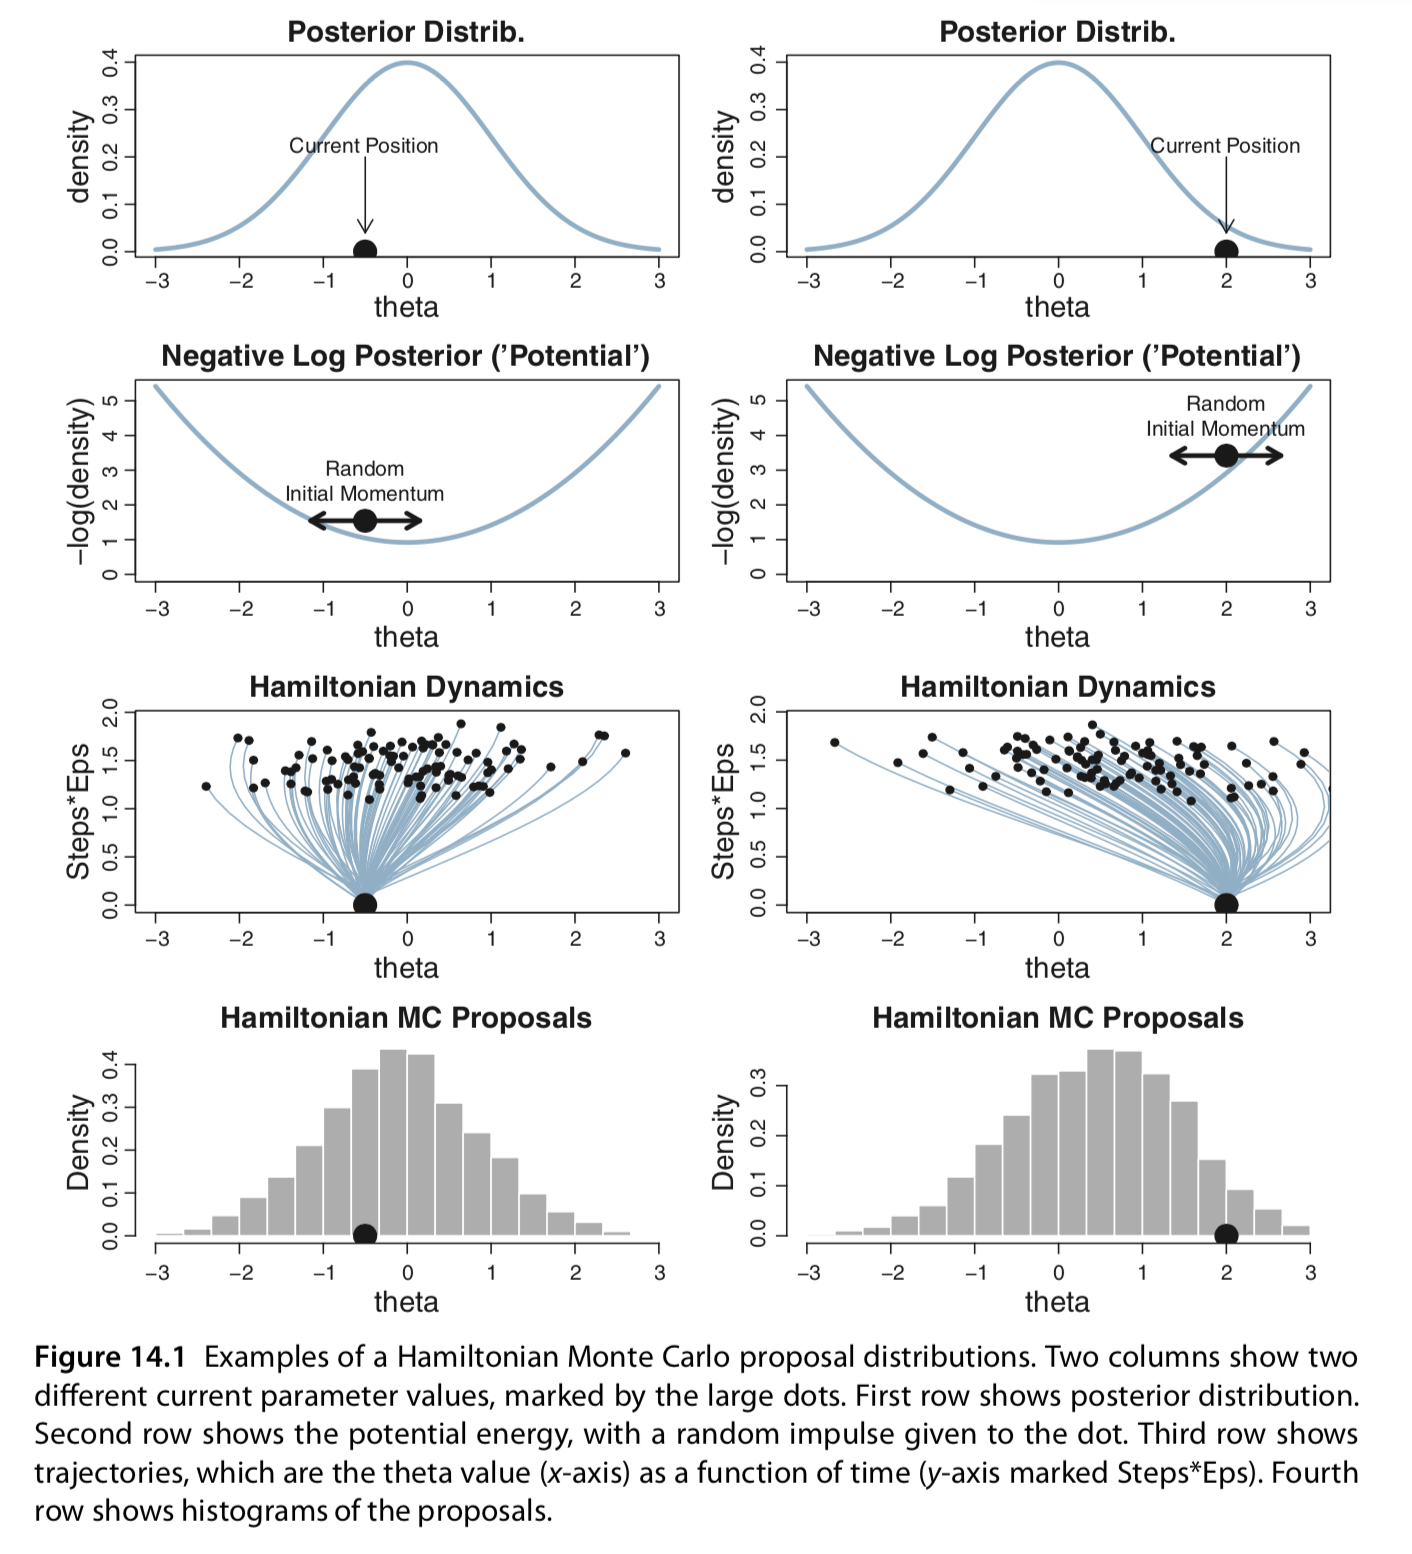
\includegraphics[width=0.8\textwidth]{potential}
        \caption{HMC proposal distributions}
        \label{fig:potential}
    \end{figure}
    \item Posterior tall $\implies$ Potential low and vice versa.
    \item Large dot represents the current position.
    \item Proposed position generated by flicking marble in \textbf{random} direction and letting it roll for some duration. 
    \item Magnitude of flick is sampled from \textbf{zero mean Gaussian } distribution. 
    \item Flick gives \textbf{momentum} to the ball. When time is up, the new position of the ball is the new proposed jump.
    \item Ball will be near the lower part of the curve i.e it will be in regions of higher posterior probability(because the curve is inverted posteior probability).
    \item \textbf{Potential} is similar to physics concept of potential energy. 
    \item Third row in figure shows many trajectories taken by the ball from it's initial position and allowed to roll for random times.(impluses is called \textbf{Steps*Eps}. Trajectories show theta value as a function of time as the ball rolls after it receives the random initial push.
    \item Bottom row shows histogram of all proposed positions. Proposal distribution \textbf{is not} centered around initial position. 
    \item Proposal distribution has moved towards the \textbf{mode} of the posterior distribution. 
    \item \textbf{Metropolis decision rule}: Used to accept or reject proposal. $\phi$ is used to denote the momentum.
    \item In ideal system, all potential energy will be converted to kintetic energy when the marble is moving and vice versa when the marble is stable i.e lossless system.
    \item For ideal system, sum of potential($-log(p(\theta|D))$ ) and kinetic($-log(p(\phi))$ will be constant, and proposal will always be rejected.
    \item \textbf{However}, because there is always some loss in energy(due to friction) in real world scenarios, proposals will not always be accepted. 
        \[
            p_{accept} = min\bigg(\frac{p\theta_{proposed}|D)p(\phi_{proposed})}{p(\theta_{current}|D)p(\phi_{current})}, 1\bigg)
        .\] 
    \item Proposal distribution can be "tuned" by:
    \begin{enumerate}
        \item adjusting step size called \textbf{epsilon(or eps)}
        \item adjusting number of steps taken.
    \end{enumerate}
    \item Step size $\implies$ Time taken to make a step. Hence, it is called \textbf{Steps*Eps}  
    \item General acceptance rate is 62\%.
    \item Acceptance rate low $\implies$ Epsilon reduced
    \item Acceptance rate high $\implies$ Epsilon increased \textbf{and} changes in number of steps to maintain trajectory duration. 
    \item Step size controls smoothness or jaggedness of trajectory.
    \item Duration(Steps*Eps) controls how far proposed steps are from the current position.
    \begin{figure}[H]
        \centering
        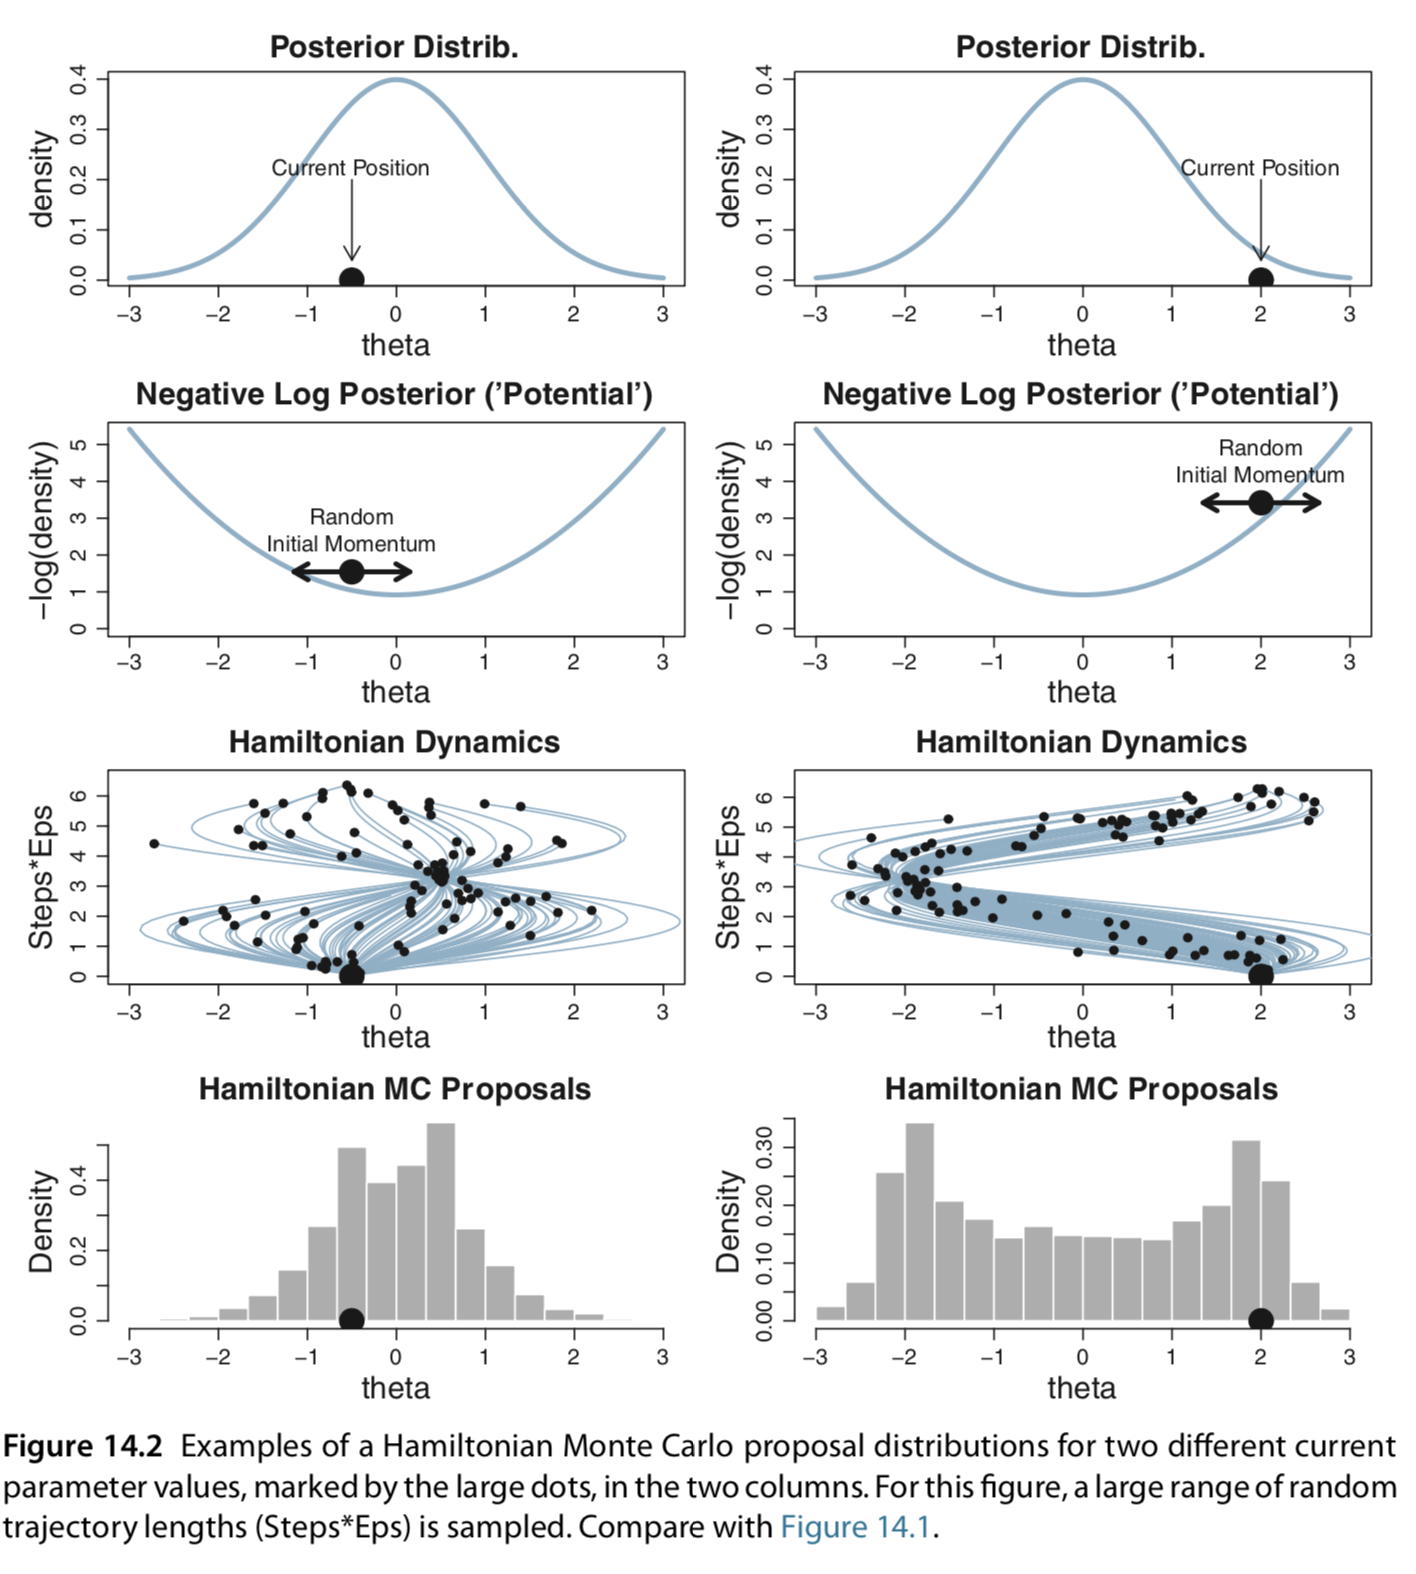
\includegraphics[width=0.8\textwidth]{trajectory_lengths}
        \caption{HMC proposal distributions for different trajectory lengths}
        \label{fig:trajectory_lengths}
    \end{figure}
    \item Duration is important because we want proposed position closer to mode of posterior distribution.
\end{itemize}
\end{document}
